% Native, editable teaching diagrams. C01--C18; no AI-generated imagery.
\begin{frame}[t]{Sensors report numbers; the state is what we infer}
\label{f:C01}
\begin{columns}[T,onlytextwidth]
\column{.48\textwidth}
\begin{tikzpicture}[every node/.style={font=\small},x=1cm,y=1cm]
\node[circle,draw=teal,fill=pale,minimum size=8mm] (n0) at (0,1.8) {0};
\node[circle,draw=teal,fill=pale,minimum size=8mm] (n1) at (3.3,1.8) {1};
\node[circle,draw=teal,fill=pale,minimum size=8mm] (n2) at (3.3,-.2) {2};
\node[circle,draw=teal,fill=pale,minimum size=8mm] (n3) at (0,-.2) {3};
\draw[arrow] (n0)--node[above] {flow 0--1}(n1);
\draw[arrow] (n1)--node[right] {flow 1--2}(n2);
\draw[arrow] (n2)--node[below] {flow 2--3}(n3);
\draw[arrow] (n0)--node[left] {flow 0--3}(n3);
\node[font=\scriptsize,above=2mm of n0] {$\theta_0=0$ reference};
\uncover<2->{\node[box,text width=4.3cm] at (1.7,-1.5) {Hidden state: three non-reference angles\\$x=[\theta_1,\theta_2,\theta_3]^T$};}
\end{tikzpicture}
\column{.49\textwidth}
\Idea{Fresh four-bus DC fixture}{Eight measurements: four flows, three injections, one angle. Three unknown angles. Redundancy permits a consistency test.}
\Question{Is a small residual the same as a trustworthy state?}
\Answer{No. We will construct two different states with the same residual.}
\small This identifiable DC example is separate from the three-phase distribution-feeder models.
\end{columns}
\Source{Classroom\_Labs L8--L9; standard\_formulations.run\_wls\_demo. State estimation: \href{https://doi.org/10.1109/TPAS.1970.292678}{Schweppe and Wildes, 1970}.}
\Bridge{What does fitting a state mean in a two-sensor example?}
\note{Start by distinguishing the network state from the sensor readings. In this small DC example, the state consists of three voltage angles relative to the reference bus. Voltage magnitudes and reactive power are outside the model. The measurements include branch flows, nodal injections and one angle reading, so they provide more equations than unknowns. That redundancy makes it possible to ask whether the readings agree with one modeled state. The arrows define branch reference directions, not necessarily actual positive power flow. Do not begin with an attack mechanism. First establish what an ordinary estimator is trying to do and what its residual means. The next two-sensor example is a separate arithmetic illustration, intentionally much simpler than this four-bus model. It lets the audience predict the estimator output before seeing matrix notation.}
\end{frame}

\begin{frame}[t]{Two equally precise sensors: find their common explanation}
\label{f:C02}
\begin{center}
\begin{tikzpicture}[node distance=1.5cm]
\node[box] (a) {sensor 1\\9 units};
\node[box,right=of a,text width=3cm] (b) {one hidden quantity $x$\\best estimate?};
\node[box,right=of b] (c) {sensor 2\\11 units};
\draw[arrow] (a)--(b);\draw[arrow] (c)--(b);
\uncover<2->{\node[box,below=.7cm of b,text width=7.2cm] (d) {$\hat x=(9+11)/2=10$\\residuals: $r=[9-10,\;11-10]^T=[-1,1]^T$};\draw[arrow] (b)--(d);}
\end{tikzpicture}
\end{center}
\Question{What mismatch remains after choosing the best common value?}
\Answer{$J=(-1)^2+1^2=2$. A residual measures mismatch to the fitted model.}
\small Illustrative scalar example: $H=[1,1]^T$, unit variance for each sensor. This is WLS with equal weights, not the four-bus run.
\Source{Original arithmetic teaching example; least-squares principle: \href{https://doi.org/10.1109/TPAS.1970.292678}{Schweppe and Wildes, 1970}.}
\Bridge{How does one inconsistent reading change the fit?}
\note{Ask the audience for the best common explanation of nine and eleven before revealing ten. Assume both sensors measure the same scalar in the same units, with equal independent noise variances of one. Under squared-error fitting, the average minimizes the sum of the two squared discrepancies. A residual is the observed reading minus the reading predicted by the fitted state. The two residuals are minus one and plus one; their squared sum is two. Explain the hat notation as an estimate rather than a true value. No detection threshold is being claimed for this arithmetic example. Its purpose is to make the estimator and residual concrete. The actual classroom network has different measurement types and variances, which later require weighting so an angle discrepancy and a flow discrepancy are compared in their own noise scales.}
\end{frame}

\begin{frame}[t]{An isolated error increases disagreement between sensors}
\label{f:C03}
\begin{columns}[T,onlytextwidth]
\column{.48\textwidth}
\Idea{Before corruption}{$z=[9,11]^T$\par $\hat x=10$\par $r=[-1,1]^T$\par $J=2$.}
\column{.48\textwidth}
\Idea{Change only sensor 1}{$z'=[15,11]^T$\par Which common estimate fits best?}
\uncover<2->{\[
\hat x'=13,\quad r'=[2,-2]^T,\quad J'=8.
\]}
\end{columns}
\begin{center}
\begin{tikzpicture}[x=.7cm]
\draw[slate,->] (8,0)--(16,0);
\foreach \x in {9,10,11,13,15}{\draw (\x,.07)--(\x,-.07);\node[below,font=\small] at (\x,-.08) {\x};}
\fill[teal] (9,0) circle (2pt);\fill[teal] (11,0) circle (2pt);
\uncover<2->{\draw[arrow,red,bend left=35] (9,.1) to node[above,font=\small] {one reading moves} (15,.1);\fill[red] (15,0) circle (2pt);}
\end{tikzpicture}
\end{center}
\footnotesize A calibrated alarm signals model inconsistency; it does not identify an attacker.
\Source{Original scalar illustration, equal unit variances. Statistical alarm assumptions are introduced on C06.}
\Bridge{What if both readings move together?}
\note{Keep the true physical quantity conceptually unchanged while modifying only the first reported number. The new readings, fifteen and eleven, are best explained by thirteen. Their residuals are plus two and minus two, so the squared mismatch rises from two to eight. This provides an intuitive reason why redundant measurements can detect some kinds of corruption: the readings no longer agree with one another as well. Do not label this arithmetic result an actual alarm, because we have not chosen a statistical threshold for this example. A larger residual can also arise from a failed sensor, incorrect topology, poor calibration or an inadequate model. An alarm indicates inconsistency under assumptions, not malicious intent. Ask what happens if both readings are changed by the same amount. That prediction prepares the central limitation without requiring matrix algebra yet.}
\end{frame}

\begin{frame}[t]{Coordinated errors can preserve the same disagreement}
\label{f:C04}
\begin{center}
\begin{tabular}{lccc}
\toprule & Measurements & Fitted state & Residual\\\midrule
Original & $[9,11]^T$ & $10$ & $[-1,1]^T$\\
Both shifted by $+3$ & $[12,14]^T$ & $13$ & $[-1,1]^T$\\\bottomrule
\end{tabular}
\end{center}
\uncover<2->{\begin{center}\large Same residual statistic: $J'=J=2$.\par\smallskip Different inferred state: $\hat x'=\hat x+3$.\end{center}}
\Idea{Consistency is not authenticity}{Both readings fit a shifted state. Consistency alone cannot recover the missing truth.}
\Question{Does LLM voting add an independent measurement?}
\Answer{No. New physical evidence must come from outside the corrupted readings.}
\Source{Original scalar adaptation of the false-data-injection principle in \href{https://doi.org/10.1145/1653662.1653666}{Liu, Ning and Reiter, CCS 2009}.}
\Bridge{How does the same idea appear in network state estimation?}
\note{This is the explicit counterexample the audience should remember. Both sensors are shifted by three, so their best common explanation shifts from ten to thirteen. Their differences from that explanation remain minus one and plus one. The residual test therefore sees exactly the same mismatch even though the inferred state has changed. The example does not require the audience to accept a complicated security claim on faith; every number can be checked mentally. Explain that the attack succeeds within this illustration because both readings can be altered coherently and there is no trustworthy independent anchor. An additional language model examining the same observations does not create that anchor. A useful agentic workflow must recognize information limits, request appropriate evidence or hold the action. The network version follows the same geometry through the measurement matrix.}
\end{frame}

\begin{frame}[t]{Weighted least squares fits the measurement model}
\label{f:C05}
\[
z=Hx+e,\qquad
\hat x=\arg\min_x (z-Hx)^T R^{-1}(z-Hx),\qquad
R=\operatorname{diag}(\sigma_1^2,\ldots,\sigma_m^2).
\]
\begin{columns}[T,onlytextwidth]
\column{.48\textwidth}
\begin{tabular}{ll}
$z\in\mathbb R^m$ & sensor measurements\\
$x\in\mathbb R^n$ & unknown state\\
$H\in\mathbb R^{m\times n}$ & linear measurement map\\
$e$ & measurement noise\\
$\sigma_j$ & channel $j$ noise scale\\
$R$ & noise covariance
\end{tabular}
\column{.48\textwidth}
\Idea{Our fresh network run}{$m=8$, $n=3$, $\operatorname{rank}(H)=3$.\par Flow $\sigma=0.004$ p.u.; injection $0.006$ p.u.; angle $0.0005$ rad.}
\uncover<2->{\small Higher precision means larger weight. Each discrepancy is normalized by its own noise scale.}
\end{columns}
\Source{Classroom\_Labs L8; standard\_formulations.weighted\_least\_squares. WLS: \href{https://doi.org/10.1109/TPAS.1970.292678}{Schweppe and Wildes, 1970}.}
\Bridge{How large is too large for the residual?}
\note{Translate each symbol into an object the audience already understands. The measurement matrix predicts sensor readings from a candidate state. The estimator chooses the state that minimizes the weighted squared disagreement. The covariance describes uncertainty in each channel; the implementation assumes independent errors, so it is diagonal. A precise channel receives more weight because a small discrepancy there is more surprising. Different measurement types may have different physical units, which is why each residual is scaled by its own standard deviation. In the fresh four-bus exercise there are eight measurements and three identifiable unknown angles. The matrix has full column rank, so the linear weighted fit has a unique state estimate. These facts make the following residual degrees-of-freedom calculation meaningful. They do not establish trustworthy provenance for the measurements or correctness of the network topology.}
\end{frame}

\begin{frame}[t]{A residual alarm is a statistical test under stated assumptions}
\label{f:C06}
\[
r=z-H\hat x,\qquad J=r^TR^{-1}r,\qquad
J>\chi^2_{m-n,\,1-\alpha}\ \Longrightarrow\ \text{alarm}.
\]
\begin{columns}[T,onlytextwidth]
\column{.48\textwidth}
\Idea{Classroom calibration}{$m-n=8-3=5$ residual degrees of freedom.\par $\alpha=0.01$; threshold $\chi^2_{5,0.99}=15.0863$.}
\column{.48\textwidth}
\uncover<2->{\Idea{Interpretation requires assumptions}{Correct linear model; full column rank; stated independent Gaussian noise and covariance. $\alpha$ is the nominal false-alarm probability.}}
\end{columns}
\Question{Does ``no alarm'' mean ``safe to control''?}
\Answer{No. It means this test found no excessive model inconsistency. Provenance and operating limits remain separate checks.}
\Source{Residual test implementation: standard\_formulations.weighted\_least\_squares. State estimation foundations: \href{https://doi.org/10.1109/TPAS.1970.292678}{Schweppe and Wildes, 1970}.}
\Bridge{Why can a coordinated shift leave this statistic unchanged?}
\note{Define the residual before defining the test statistic. Each squared residual is normalized by its variance, producing a dimensionless sum. With a correct full-rank linear model and independent Gaussian errors of the stated covariance, the statistic follows a chi-square distribution with the number of measurements minus the number of estimated states degrees of freedom. Here that is five. A one-percent upper-tail threshold is about fifteen point zero nine. This is a calibration statement under assumptions, not a guarantee in an arbitrary real network. An alarm can reflect model error or ordinary sensor failure. Conversely, a missing alarm cannot establish that data are authentic. Ask participants to recall the two sensors shifted together. The next slide shows why that arithmetic example extends exactly to a family of coordinated changes in the linear network model.}
\end{frame}

\begin{frame}[t]{The cancellation is visible in three lines}
\label{f:C07}
\begin{align*}
\text{Coordinated measurement change:}\qquad z'&=z+Hc,\\[7pt]
\uncover<2->{\text{New WLS estimate:}\qquad\hat x'&=\hat x+c,}\\[7pt]
\uncover<3->{\text{New residual:}\qquad r'&=z+Hc-H(\hat x+c)=z-H\hat x=r.}
\end{align*}
\small $c\in\mathbb R^n$: chosen state shift; $a=Hc$: coordinated change to sensor readings. Therefore $J'=J$ with unchanged covariance.
\Idea{The assumptions are part of the result}{Full-rank linear WLS; correct knowledge of $H$; ability to alter the required unprotected channels. A protected channel can restrict feasible shifts.}
\Question{Which term disappears when we subtract the predicted measurements?}
\uncover<3->{\textcolor{teal}{The added $Hc$ cancels exactly.}}
\Source{False-data-injection construction: \href{https://doi.org/10.1145/1653662.1653666}{Liu, Ning and Reiter, CCS 2009}. Defensive four-bus exercise in L8.}
\Bridge{Can your experiment reproduce equal residuals but different state errors?}
\note{Reveal the three lines separately and pause before the last cancellation. The vector c is a change in the inferred state, and multiplying it by H produces the corresponding change in all modeled sensor readings. For full-rank linear weighted least squares with the same weights, adding this measurement change shifts the fitted state by c. Subtracting the new predicted readings removes the same added term, leaving the original residual. No mysterious failure of the numerical solver is involved; it solves the altered measurement problem correctly. State the attack assumptions instead of implying that every real system permits this construction. The exercise assumes knowledge of the model and control of all required unprotected readings. Protected independent channels can prevent some shifts from being consistent. The following experiment is confined to a synthetic educational DC model.}
\end{frame}

\begin{frame}[fragile,t]{Hands-on: sweep isolated and coordinated corruption}
\label{f:C08}
\Checkpoint{L8}{Seven minutes: run the full cell; compare residual and state-error plots.}
\lstinputlisting[style=python,firstline=1,lastline=5]{snippets/L8.py}
\begin{columns}[T,onlytextwidth]
\column{.48\textwidth}
\Idea{Predict first}{For a growing isolated bias, what happens to $J$? For a growing $Hc$ shift, what happens to $J$ and the state error?}
\column{.48\textwidth}
\uncover<2->{\Idea{Read two different quantities}{The residual is observable from measurements and the model. State error uses simulated truth and is an offline evaluation metric.}}
\end{columns}
\small The scale multiplies a synthetic perturbation. It is not an estimate of attack likelihood or real-world severity.
\Source{Exact excerpt: Classroom\_Labs L8 lines 1--5. Fixed synthetic seeds and attack directions in src/classroom\_labs.py and standard\_formulations.py.}
\Bridge{Which curve can an operator compute without knowing the truth?}
\note{Give participants the full seven minutes to run and inspect the experiment. The attack scale varies over five stated values for both isolated corruption and the coordinated Hc construction. Ask them to predict the two plots before looking at the table. Their explanation should distinguish a detector output from an evaluation metric. The residual statistic can be computed from the reported measurements and the assumed model. The norm of state error requires the true simulated state, which is available to us because this is an experiment. A real operator does not generally know that truth. Do not let the workflow use offline truth as if it were an available verification signal. Participants should record one example where no residual alarm occurs despite a changed inferred state, and explain why additional independent information would be required.}
\end{frame}

\begin{frame}[t]{Same residual does not imply the same state}
\label{f:C09}
\begin{center}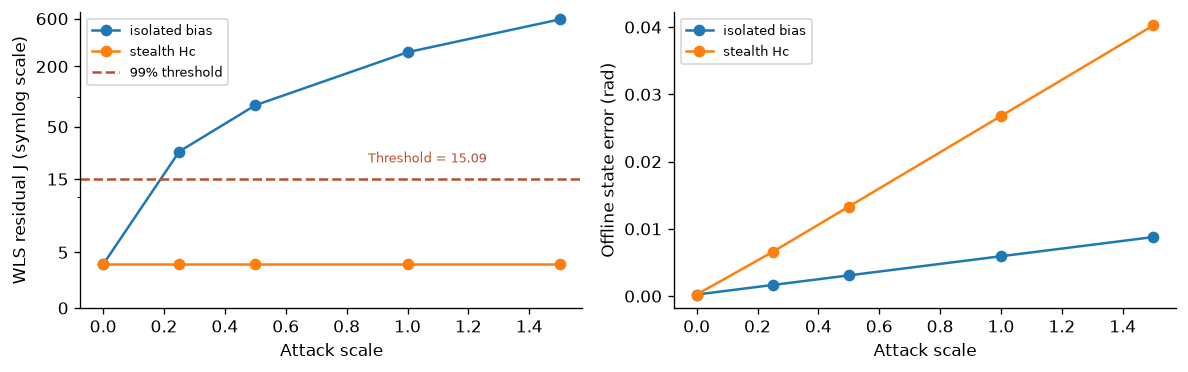
\includegraphics[width=.88\linewidth,height=3.65cm,keepaspectratio]{figures/classroom_cyber.png}\end{center}
\small At scale 1: isolated-corruption $J\approx277.50$; coordinated-shift $J\approx3.92$. Threshold $15.09$.
\uncover<2->{\Idea{Keep the metrics separate}{Left: consistency evidence available to the estimator. Right: state error against simulated truth, used only to evaluate the experiment.}}
\Source{Original computed figure: Classroom\_Labs L8 / classroom\_cyber.png. Coordinated $J\approx3.92022$ remains constant across the sampled scales.}
\Bridge{What should Awareness report when consistency passes but trust is unresolved?}
\note{Read the plots in order. The residual plot shows that a sufficiently large isolated perturbation violates the consistency test, while the coordinated construction retains the original statistic at every sampled scale. The state-error plot reveals that the coordinated corruption still changes the inferred state. Mention the residual-axis scaling shown on the figure so students do not interpret vertical distances as an ordinary linear scale. At scale one, the isolated statistic is about two hundred seventy-seven, well above fifteen, while the coordinated statistic remains about three point nine. Those are reproducible outcomes for the stated synthetic seeds and model, not general attack-detection rates. The right-hand plot is an offline scientific audit using known truth. The next workflow decision must instead rely on information actually available to the estimator and the declared provenance assumptions.}
\end{frame}

\begin{frame}[t]{Awareness must distinguish consistency from trustworthy provenance}
\label{f:C10}
\begin{center}
\begin{tikzpicture}[node distance=.65cm]
\node[box,text width=3.3cm] (a) {Residual test\\Do readings fit the model?};
\node[box,text width=3.3cm,right=of a] (b) {Provenance check\\Which channels are trusted?};
\node[box,text width=3.3cm,right=of b] (c) {Control decision\\Enough evidence to act?};
\draw[arrow] (a)--(b);\draw[arrow] (b)--(c);
\end{tikzpicture}
\end{center}
\Idea{A legitimate output is HOLD}{If measurements are suspect and no trustworthy replacement is available, request evidence instead of manufacturing a confident state estimate.}
\Question{Can an LLM vote resolve missing observability or missing trusted channels?}
\Answer{No. Voting over the same evidence does not add an independent physical constraint.}
\Source{Information limitation illustrated by \href{https://doi.org/10.1145/1653662.1653666}{Liu et al., 2009}; explicit protected-channel assumption in Classroom\_Labs L9.}
\Bridge{What replacement information is assumed in the recovery exercise?}
\note{This slide places the statistical lesson inside the agentic workflow. Awareness should produce separate fields for residual consistency and measurement provenance. A low residual supports only the first field. If a cyber incident or external evidence makes the measurements suspect, the workflow should ask whether trustworthy replacement channels exist and whether they make the state identifiable. The language model can summarize the missing evidence, request an authorized tool or explain why the action is held. It cannot create a trustworthy measurement by reasoning more fluently. Multiple model responses based on the same corrupted data have the same information limitation. The exercise deliberately includes a HOLD branch when replacement channels are unavailable. This is not a claim that the residual test itself detects the stealth case; that would contradict the counterexample we just demonstrated.}
\end{frame}

\begin{frame}[t]{Recovery assumes three independent protected angle readings}
\label{f:C11}
\[
z_T=H_Tx+e_T,\qquad H_T=I_3,\qquad
\sigma_T=0.00005\ \text{rad per channel}.
\]
\begin{center}
\begin{tikzpicture}[node distance=.65cm]
\node[box,text width=2.7cm] (a) {protected $\theta_1$};
\node[box,text width=2.7cm,right=of a] (b) {protected $\theta_2$};
\node[box,text width=2.7cm,right=of b] (c) {protected $\theta_3$};
\uncover<2->{\node[box,text width=8.2cm,below=.65cm of b] (d) {Rank 3: recover three angles.\\Exactly determined: zero residual degrees of freedom.};\draw[arrow] (a)--(d);\draw[arrow] (b)--(d);\draw[arrow] (c)--(d);}
\end{tikzpicture}
\end{center}
\small Subscript $T$: trusted set; $I_3$: identity matrix; $e_T$: assumed measurement noise.
\Idea{An assumption, not an implemented security protocol}{Authentication and physical protection are external requirements. This three-channel fit provides no redundant chi-square detection test.}
\Source{Exact classroom recovery model: standard\_formulations.run\_wls\_demo; Classroom\_Labs L9. Protected measurements are assumed trustworthy.}
\Bridge{How can a trusted estimate support a constrained corrective action?}
\note{Be explicit that the recovery channels are assumed, not discovered by the LLM or authenticated by this notebook. There are three independent angle readings, one for each unknown angle, with the stated small noise level. The identity measurement matrix has rank three, so the state is identifiable from this trusted set. However, three measurements for three unknowns leave zero residual degrees of freedom. The estimator can fit them exactly, so it has no redundant chi-square test for detecting an error within this set. Trust must come from the external measurement and security assumptions. This distinction prevents the recovery demonstration from becoming a circular claim that a zero residual proves security. Ask participants what additional engineering would be needed to establish that trust in practice. The tutorial then uses the recovered estimate for a small constrained redispatch calculation.}
\end{frame}

\begin{frame}[t]{Corrective control: move a stressed flow back inside its limit}
\label{f:C12}
\begin{columns}[T,onlytextwidth]
\column{.49\textwidth}
\begin{tikzpicture}[x=15cm,y=1cm]
\draw[slate,->] (0,0)--(.29,0);
\foreach \x in {.17,.18,.24}{\draw (\x,.1)--(\x,-.1);}
\node[font=\scriptsize,below] at (.24,-.12) {0.24};
\draw[slate] (.17,-.12)--(.12,-.45);
\node[font=\scriptsize,below] at (.12,-.45) {target 0.17};
\draw[red,dashed,thick] (.18,-.1)--(.18,1);
\node[font=\small,above] at (.18,1) {limit 0.18};
\fill[red] (.24,0) circle (2.4pt);
\uncover<2->{\draw[arrow,bend right=25] (.24,.15) to node[above,font=\small] {flexible injection $u$} (.17,.15);\fill[teal] (.17,0) circle (2.4pt);}
\end{tikzpicture}
\column{.48\textwidth}
\Idea{Noiseless arithmetic illustration}{For branch 1--2, suppose estimated flow is $0.24$ p.u. and sensitivity is $-4/7$.\par A $0.01$ p.u. margin gives target $0.17$.\par\smallskip $u\ge(0.24-0.17)/(4/7)=0.1225$ p.u.}
\end{columns}
\small $u$: injection at node 2, balanced by the reference source. The actual noisy protected-state run gives $u\approx0.12169$ p.u.; the illustration above is not that exact solve.
\Source{Sensitivity $F B^{-1}[0,1,0]^T$ from standard\_formulations.\_redispatch. Original noiseless arithmetic illustration; all quantities here are per unit.}
\Bridge{How do we choose the smallest admissible correction across all branches?}
\note{Before showing a quadratic program, make the control action concrete. An injection at node two, balanced by the reference source, changes branch flows through a known DC sensitivity. For the stressed branch, the sensitivity is minus four-sevenths. In this separate noiseless illustration, an estimated flow of zero point two four must be brought to zero point one seven to preserve a zero point zero one margin below the physical zero point one eight limit. Dividing the needed flow reduction by the sensitivity magnitude gives a minimum injection of zero point one two two five. The real classroom solve uses a noisy protected estimate, so its optimum is slightly different. Label that distinction carefully. The diagram does not use simulated truth as an operational gate; it simply teaches how a linear flow sensitivity becomes an action constraint.}
\end{frame}

\begin{frame}[fragile,t]{Planning uses a constrained quadratic control problem}
\label{f:C13}
\[
\min_{0\le u\le0.5}\ \tfrac12u^2
\quad\text{s.t.}\quad
\left|F\hat x_T+b_u u\right|\le\ell-\delta\mathbf1,
\qquad b_u=FB^{-1}e_2.
\]
\small
$F$: angle-to-flow map; $B$: non-reference nodal injection matrix; $e_2=[0,1,0]^T$; $\hat x_T$: trusted estimate; $b_u$: flow sensitivity.\par
$\ell=[0.35,0.18,0.35,0.35]^T$ p.u.: branch limits; $\delta=0.01$ p.u.: planning margin; $\mathbf1$: vector of ones. Absolute values and inequalities are componentwise.
\Checkpoint{L9}{Run both evidence conditions with the same numerical control method.}
\lstinputlisting[style=python,firstline=1,lastline=2]{snippets/L9.py}
\uncover<2->{\Idea{Method and acceptance}{SLSQP solves this scalar convex QP. Independent post-solve bounds and predicted-flow checks can still return HOLD.}}
\Source{Exact excerpt: Classroom\_Labs L9 lines 1--2; constrained model and checks in standard\_formulations.\_redispatch. DC illustration, not AC feeder resilience.}
\Bridge{What changes when trusted replacement channels are unavailable?}
\note{Read the objective as choosing the smallest squared corrective injection. The constraints keep all predicted branch-flow magnitudes within their ratings minus the engineering margin, and restrict the injection to its allowed interval. Define every matrix by its role instead of asking students to memorize the notation. The vector e-two selects injection at the second non-reference node, while the reference source balances the change. For this fixed linear model, the resulting scalar problem is convex. The implementation uses SLSQP and independently checks finite values, action bounds and predicted flow constraints after solving. The protected estimate is an input with an explicit trust assumption. The two code lines compare that assumption being available or unavailable; they do not change the numerical control objective. This distinguishes an information gate from a contest between optimization algorithms.}
\end{frame}

\begin{frame}[t]{Hands-on: evidence availability changes the permitted response}
\label{f:C14}
\Checkpoint{L9}{Five minutes: run the full cell; identify the acceptance assumption.}
\begin{center}
\begin{tabular}{lcc}
\toprule Condition & Response & Flexible injection\\\midrule
No trusted replacement channels & HOLD & none proposed\\
Three protected angles assumed & PROPOSE & $0.12169$ p.u.\\\bottomrule
\end{tabular}
\end{center}
\uncover<2->{\Idea{Two checks, with different information}{Predicted branch 1--2 flow: $0.17000$ p.u. (operational model check).\par Actual simulated flow: $0.17046<0.18$ p.u. (offline truth audit).}}
\Question{Why is the offline value not an input to the operator's verification rule?}
\Answer{The real system does not reveal its exact state just because our simulator knows it.}
\Source{Fresh L9 output with fixed synthetic seeds; standard\_formulations.run\_wls\_demo. The zero-violation offline audit applies to this modeled case only.}
\Bridge{How does the five-stage workflow carry this distinction?}
\note{Allow five minutes for the full cell and discussion. The no-trust condition returns HOLD rather than an invented replacement state. The protected condition proposes a flexible injection of about zero point one two one six nine per unit. The predicted stressed-branch flow is at the zero point one seven planning target. When the experiment separately evaluates that same action against its known true state, the actual modeled flow is about zero point one seven zero four six, still below the physical limit. These numbers have different roles. Predicted constraints support the candidate under the trusted-estimate assumption. Truth-based flow and violation count are offline performance audits. A successful audit on one seeded example is not a robustness guarantee against arbitrary measurement error or model mismatch. Ask participants to state the protected-channel assumption in their own words before moving on.}
\end{frame}

\begin{frame}[t]{Every stage has a specific numerical or evidentiary job}
\label{f:C15}
\small
\renewcommand{\arraystretch}{1.12}
\begin{tabularx}{\linewidth}{>{\bfseries\raggedright\arraybackslash}p{2.35cm}>{\raggedright\arraybackslash}p{4.4cm}>{\raggedright\arraybackslash}X}
\toprule Stage & Specific method & Inspectable output\\\midrule
Awareness & WLS, residual and trust checks & Alarm, rank, provenance status\\
Planning & Constrained DC redispatch QP & Injection and predicted flow margins\\
Simulation & DC flow calculation & Response to the candidate injection\\
Verification & Provenance and limit gates & PROPOSE or HOLD, with failed condition\\
LLM Optimizer & Allowed refinement selection & New tool request and returned rationale\\\bottomrule
\end{tabularx}
\uncover<2->{\Idea{Use the method suited to the decision}{WLS estimates the state; the QP selects the correction. L10 replays the archived five-stage language trace.}}
\Source{Classroom\_Labs L8--L10; archived cyber\_stealth / dc run in proposal\_complete\_workflow.json. Fresh numerical fixtures and archived LLM calls are separately labeled.}
\Bridge{What does the actual Llama refinement response look like?}
\note{Return to the five-stage vocabulary after the audience understands the numerical problem. Awareness computes an estimate and a consistency statistic, but also records rank and trust conditions. Planning solves the constrained redispatch problem only when its required inputs are admissible. Simulation evaluates the action in the stated DC model. Verification checks provenance and modeled limits and can hold the recommendation. The language optimizer may select from permitted refinements and request another simulation; it cannot waive those gates. This case uses a quadratic program because that is the natural form of the stated decision. It would be misleading to label every calculation MPC or DRL for consistency of branding. L8 and L9 are fresh numerical exercises, while L10 supplies the full archived language trace. That distinction keeps live execution, replayed evidence and conceptual stage roles honest.}
\end{frame}

\begin{frame}[t]{Actual Llama response: request a new checked candidate}
\label{f:C16}
\small
\Idea{Planning, 0.829 s}{\textit{``Requesting new candidates based on the given tools and objective.''}}
\uncover<2->{\Idea{LLM Optimizer selects TRUSTED\_QP, 1.195 s}{\textit{``The current lowest-cost candidate E03 has a cost of 0.008671610999497877, but the permitted refinement TRUSTED\_QP offers a new approach to minimize the objective. Selecting this operation will request a new simulation and verification.''}}}
\uncover<3->{\begin{center}\textbf{Numerical result:} $u=0.12169$ p.u., cost $0.00740467$.\par Acceptance still depends on trusted-input and flow-limit gates.\end{center}}
\Source{Exact returned rationale fields: archived cyber\_stealth / dc trace, proposal\_complete\_workflow.json. Model-call wall times; rounded only outside quotes.}
\Bridge{Does this language-guided refinement outperform the matched fixed supervisor?}
\note{Present these as observable response fields from the saved trace, not as access to hidden internal reasoning. The short planning reply requests candidates. The optimizer reply selects a permitted trusted-QP refinement and explicitly asks for another simulation and verification. The reported model-call times are about eight hundred twenty-nine milliseconds and one point one nine five seconds in the archived environment. The final numerical result comes from the constrained solver and its checks, not from the prose. The response does not prove that the trusted measurements are authentic, that the DC model is adequate for a distribution feeder, or that an operator has authorized execution. Those remain separate conditions. This example shows where a language response can help explain a workflow step while leaving authority with defined tools, evidence and approval. The next slide tests the final outcome against the fixed supervisor.}
\end{frame}

\begin{frame}[t]{A matched baseline avoids crediting the LLM for better information}
\label{f:C17}
\begin{center}
\begin{tabular}{lrr}
\toprule Archived DC cyber response & Fixed supervisor & Llama supervisor\\\midrule
Flexible injection (p.u.) & 0.12169 & 0.12169\\
Objective $\tfrac12u^2$ & 0.00740467 & 0.00740467\\
Total elapsed time (s) & 0.00381 & 5.203\\\bottomrule
\end{tabular}
\end{center}
\uncover<2->{\Idea{What actually enabled recovery?}{The trusted measurement assumption plus constrained numerical control. Llama added tool-selection language and a trace; it did not improve this recorded optimum.}}
\Question{Would comparing untrusted baseline data with trusted agent data be fair?}
\Answer{No. That would mix the value of additional information with the value of orchestration.}
\Source{ARCHIVED ACTUAL: fixed versus agentic cyber\_stealth / dc, proposal\_complete\_workflow.json. Same objective and evidence assumptions; one recorded run, four Llama calls.}
\Bridge{What should the operator see when the workflow finishes?}
\note{The fixed and Llama supervisors reach the same action and objective in this archived DC case. Their total elapsed times differ substantially, with the fixed supervisor completing in a few milliseconds and the language-guided workflow taking about five seconds. These are single-run measurements, not distributions or universal performance claims. The comparison is meaningful because the numerical objective, tools and evidence assumptions are matched. If the baseline had only corrupted measurements while the agent received protected measurements, any benefit would combine better information with orchestration. Avoid making that unfair attribution. The scientific lesson is that protected information and constrained control enable the recovery in this example. The agentic layer can organize requests, reasons, holds and evidence, but its additional value should be evaluated through explicit workflow and human-performance measures, alongside its latency and failure modes.}
\end{frame}

\begin{frame}[t]{The control-room handoff is a decision packet, not a green badge}
\label{f:C18}
\begin{columns}[T,onlytextwidth]
\column{.49\textwidth}
\Idea{What the operator sees}{Proposed action and objective.\par Sensor trust and model scope.\par Current revision and failed/passed checks.\par Measured latency and available alternatives.}
\column{.47\textwidth}
\begin{tikzpicture}[node distance=.55cm]
\node[box,text width=4.3cm] (a) {Evidence-backed recommendation};
\node[box,text width=4.3cm,below=of a] (b) {Acknowledge \quad Revise \quad Reject};
\node[box,text width=4.3cm,below=of b] (c) {Read back the resulting state};
\draw[arrow] (a)--(b);\draw[arrow] (b)--(c);
\end{tikzpicture}
\end{columns}
\Question{What did the three cases teach about choosing numerical methods?}
\Answer{Continuous voltage control, discrete restoration and evidence-limited cyber response need different tools within one auditable workflow.}
\Source{Case synthesis: Classroom\_Labs L1--L10; operator readback exercise L12. The tutorial dashboard is an educational interface, not a deployed control system.}
\Bridge{How should we evaluate usefulness, reliability and operator effort together?}
\note{End the cyber chapter by returning to the operator rather than to an optimizer score. A useful recommendation includes its proposed action, the objective, the measurement trust assumptions, the model used, the relevant revision and the outcome of each required check. The operator can then acknowledge, revise or reject it. After any authorized action, readback should establish what state was actually reached; an acknowledgment alone is not physical confirmation. Across the three cases, the numerical tools differ because the decisions differ. Voltage support uses continuous-control methods, restoration adds discrete topology and pickup choices, and cyber response exposes information and provenance limits before constrained control. The common agentic framework is a disciplined flow of requests, tools, checks and human decisions. The closing section will evaluate that workflow without confusing documentation quality with electrical performance or claiming unmeasured benefits.}
\end{frame}
